\documentclass[12pt,a4paper]{article}
\usepackage[utf8]{inputenc}
\usepackage[T2A]{fontenc}
\usepackage[russian]{babel}
\usepackage{amsmath,amssymb}
\usepackage{graphicx}
\usepackage{booktabs}
\usepackage{multirow}
\usepackage{geometry}
\usepackage{float}
\usepackage{eso-pic}
\graphicspath{{./}}

\geometry{top=2cm,bottom=2cm,left=2.5cm,right=1.5cm}

\title{\textbf{Лабораторная работа 1.3.1}\\
Определение модуля Юнга на основе исследования деформации растяжения}

\author{
    Студент \underline{Шеховцов Василий Максимович}\\
    Группа \underline{Б03-601}\\
    Преподаватель \underline{Ивлев Д.А.}
}

\date{
Московский Физико-технический институт\\
(национальный исследовательский университет)\\
30 сентября 2026 г.
}

\begin{document}

\AddToShipoutPictureFG*{
    \AtPageUpperLeft{
        \hspace{1.5cm}
        \raisebox{-1cm}{
            \makebox[0pt][l]{Шеховцов В.М.}
        }
    }
}

\maketitle

\section*{Цель работы}
Экспериментально получить зависимость между напряжением и деформацией(закон Гука) при помощи
одноосного растяжения; по результатам измерений вычислить модуль Юнга.

\section*{Оборудование}
\begin{itemize}
    \item Прибор Лермантова
    \item проволока из исследуемого материала
    \item зрительная труба со шкалой
    \item набор грузов
    \item микрометр
    \item рулетка
\end{itemize}

\section*{1.Теоретические сведения}
Растяжение проволоки соответствует напряженному состоянию вдоль одной оси, которое описывается формулой:
\begin{equation}
    \frac{F}{S} = E \cdot \frac{\Delta l}{l}
\end{equation}
Эту формулу можно перезаписать в следующем виде:
\begin{equation}
    F = k \Delta l
\end{equation}
где $k = \frac{ES}{l}$ - коэффициент жесткости проволоки, который зависит от материала, длины и площади поперечного сечения проволоки.

Для определения модуля Юнга используется прибор Лермантова, схема которого изображена на рис. 1
. Верхний конец проволки П, изготовленной из исследуемого материала, прикреплен к консоли К, а нижний - 
к цилиндру, которым оканчивается шарнирный кронштейн Ш. На этот же цилиндр опирается рычаг $r$, связанный с зеркальцем З. Таким образом,
удлинение проволоки можно измерить по углу поворота зеркальца.

Натяжение проволоки можно менять, перекладывая грузы с площадки М на площадку О и наоборот. Такая система позволяет исключить влияние деформации кронштейна К на точность
измерений, так как нагрузка на нем время время остается постоянной.

При проведении эксперимента неоьходимо учитывать, что проволока П всегда несколько изогнута, что не может не сказаться на результатах, особенно при небольших нагрузках.
Проволока вначале не столько растягивается, сколько выпрямляется.

\begin{figure}[H]
    \centering
    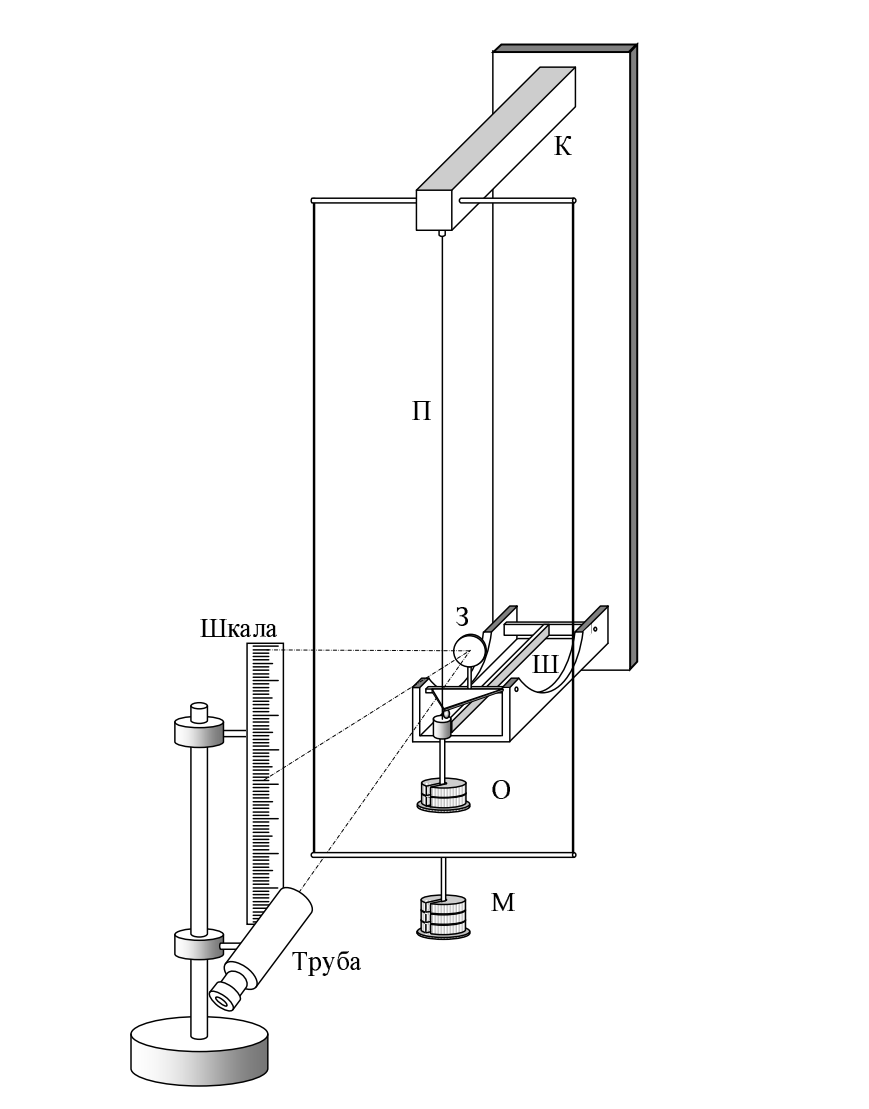
\includegraphics[width=0.8\textwidth]{map1.png}
    \caption{Прибор Лермантова}
    \label{fig:metka}
\end{figure}

Направим зрительную трубу на зеркальце. Так как мы считаем проволоку слабо растяжимой, то 
$\Delta l \ll r$. Причем угол наклона к горизонтали можно найти по формуле $\alpha = \frac{\Delta l}{r}$. Также при помощи 
геометрической оптики угол можно выразить как $\alpha = \frac{n}{2h}$, где $n$ - изменение показания шкалы относительно начального, а $h$ - расстояние от шкалы до зеркальца. Таким образом, получаем формулу для определения удлинения проволоки:
\begin{equation}
    \Delta l = \frac{nr}{2h}
\end{equation}
В нашей установке отсчёты по шкале при увеличении нагрузки уменьшаются (направление счёта определяется подписью шкалы и положением зрительной трубы), поэтому удлинение вычисляется по модулю изменения показания: $\Delta l = |n_i - n_1|\,\dfrac{r}{2h}$.

Значит, формулу (1) можно переписать в виде:
\begin{equation}
    \frac{F}{S} = E \cdot \frac{nr}{2hl}    
\end{equation}


\section*{2. Измерение и обработка данных}
1. Получим таблицу с характеристиками установки
\begin{table}[H]
    \centering
    \caption{Параметры установки}
    \label{tab:metka}
    \begin{tabular}{|c|c|c|c|c|}
        \hline
        $d_{\text{пр}}$, мм & $r$, мм & $l$, мм & $h$, мм & $\sigma_{\text{пр}}$, Н/мм² \\
        \hline
        $0.51 \pm 0.01$ & $20 \pm 1$ & $133.0 \pm 0.5$ & $176 \pm 0.5$ & 900 \\
        \hline
    \end{tabular}
\end{table}
2. Рабочее напряжение не должно превышать 30\% от величины разрушающего. Оценим,
сколько грузов можно подвесить к проволоке. Найдем площадь:
\[
    S = \frac{\pi d^2}{4} = 0.204 \text{ мм²}
\]
\[
\sigma_S = 2S \frac{\sigma_d}{d} = 0.008 \text{ мм²}
\]
Максимальная нагрузка, которую можно подвесить к проволоке:
\[
    P_{\text{max}} = 0.3 \sigma_{\text{пр}} S = 55.1 \text{ Н}
\]
\[
    \sigma_{P_{\text{max}}} = 0.3 \sigma_{\text{пр}} \sigma_S = 0.7 \text{ Н}
\]
3. Проверим данную оценку на практике. Будем подвещивать по одному грузику за раз и
наблюдать за показанием шкалы прибора. Деформация была замечана при подвешивании 5 грузов.

4. Начнем основной эксперимент, будем последовательно класть грузы, потом поочередно снимать. Сделаем 2 серии и получим таблицу:
\begin{table}[H]
    \centering
    \caption{Параметры установки}
    \label{tab:params}
    \begin{tabular}{|c|c|c|c|c|c|}
        \hline
        $\Delta m$, г & $P$, Н & $n_{1,\text{вниз}}$, см & $n_{1,\text{вверх}}$, см & $n_{2,\text{вниз}}$, см & $n_{2,\text{вверх}}$, см \\
        \hline
        245.2 & 2.41 & 27.4 & 31.0 & 28.2 & 14.4 \\
        \hline
        245.5 & 4.81 & 25.6 & 28.8 & 26.4 & 16.2 \\
        \hline
        245.8 & 7.23 & 23.9 & 26.8 & 24.7 & 17.7 \\
        \hline
        245.3 & 9.63 & 22.5 & 25.0 & 22.9 & 19.4 \\
        \hline
        245.5 & 12.04 & 20.8 & 23.2 & 21.7 & 21.1 \\
        \hline
        245.8 & 14.45 & 19.7 & 21.5 & 19.6 & 22.9 \\
        \hline
        245.2 & 16.86 & 17.8 & 19.7 & 17.8 & 24.7 \\
        \hline
        245.3 & 19.26 & 16.2 & 18.0 & 16.7 & 26.5 \\
        \hline
        245.9 & 21.68 & 14.6 & 16.8 & 14.5 & 28.4 \\
        \hline
        245.3 & 24.08 & 13.2 & 14.7 & 12.7 & 30.4 \\
        \hline
    \end{tabular}
\end{table}
Нагрузка $P$ рассчитана как вес всех грузов, лежащих на площадке: $P = g\sum \Delta m$, где $g = 9.81$ м/с². Массы грузов заданы с точностью 0.1 г, относительная погрешность $P$ составляет около 0.05\% и далее не учитывается.

6. Построим график зависимости удлинения проволоки $\Delta l$ от нагрузки $P$. Удлинение рассчитаем по формуле (3). Нулевое показание шкалы не использовалось, так как в начале нагружения проволока не столько растягивается, сколько выпрямляется. Поэтому $\Delta l$ отсчитывается от показания при первой нагрузке $P_1 = 2.41$ Н: $\Delta l_i = |n_i - n_1|\,\dfrac{r}{2h}$. Максимальная нагрузка $24.08$ Н не превышает расчётного значения $P_{\text{max}} = 55.1$ Н. Для серии 2 при разгрузке показания в таблице идут в порядке снятия грузов, поэтому они сопоставлены нагрузкам в обратном порядке (последняя строка соответствует нулевой нагрузке и не использована).

\begin{table}[H]
    \centering
    \caption{Удлинение проволоки $\Delta l$, мм}
    \label{tab:dl}
    \begin{tabular}{|c|c|c|c|c|}
        \hline
        $P$, Н & серия 1, нагружение & серия 1, разгрузка & серия 2, нагружение & серия 2, разгрузка \\
        \hline
        2.41 & 0.000 & 0.000 & 0.000 & 0.000 \\
        \hline
        4.81 & 0.102 & 0.125 & 0.102 & 0.108 \\
        \hline
        7.23 & 0.199 & 0.239 & 0.199 & 0.210 \\
        \hline
        9.63 & 0.278 & 0.341 & 0.301 & 0.312 \\
        \hline
        12.04 & 0.375 & 0.443 & 0.369 & 0.415 \\
        \hline
        14.45 & 0.438 & 0.540 & 0.489 & 0.511 \\
        \hline
        16.86 & 0.545 & 0.642 & 0.591 & 0.608 \\
        \hline
        19.26 & 0.636 & 0.739 & 0.653 & 0.693 \\
        \hline
        21.68 & 0.727 & 0.807 & 0.778 & 0.795 \\
        \hline
        24.08 & 0.807 & 0.926 & 0.881 & 0.823 \\
        \hline
    \end{tabular}
\end{table}

\begin{figure}[H]
    \centering
    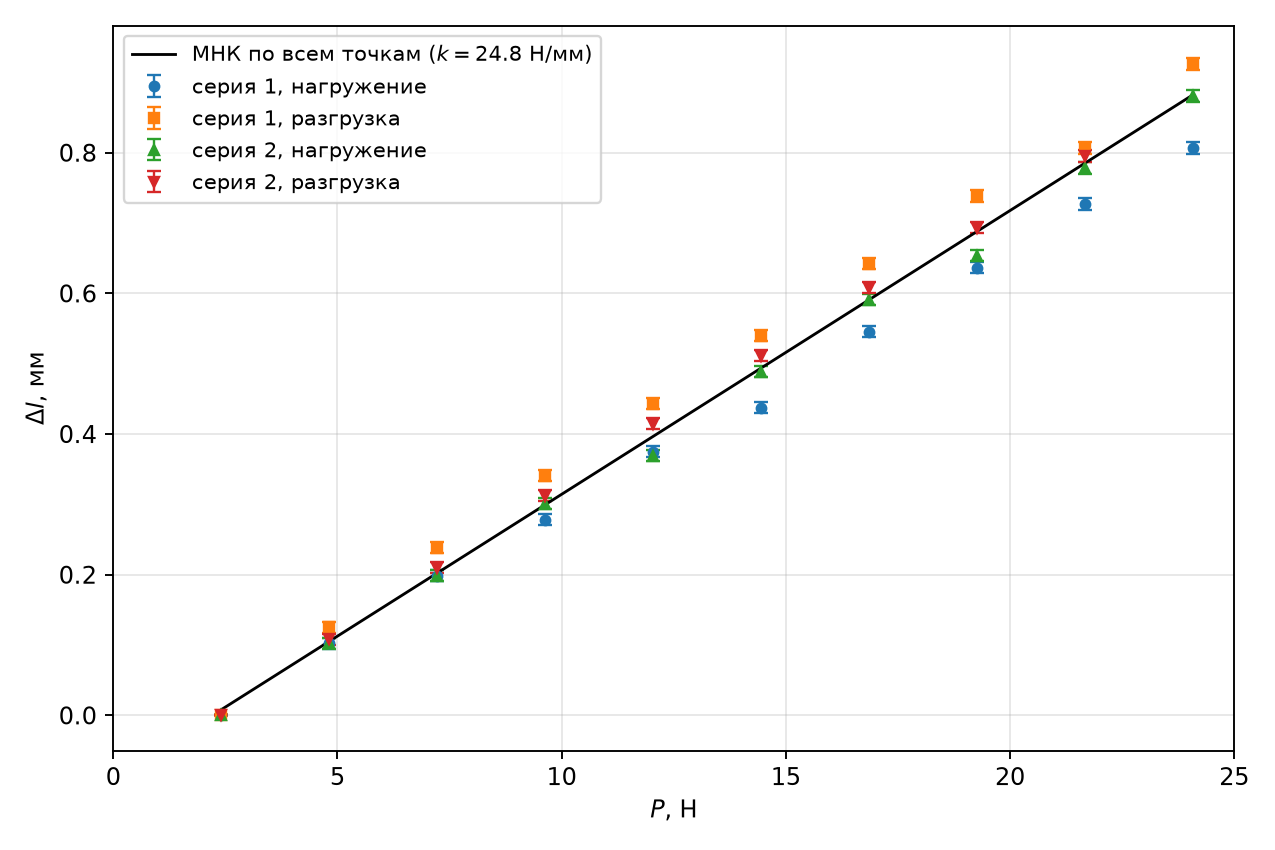
\includegraphics[width=0.85\textwidth]{graph.png}
    \caption{Зависимость удлинения проволоки $\Delta l$ от нагрузки $P$. Прямая --- аппроксимация методом наименьших квадратов по всем точкам}
    \label{fig:graph}
\end{figure}

Точки в пределах разброса ложатся на прямую, то есть выполняется закон Гука $F = k\Delta l$. Коэффициент жёсткости $k$ найдём методом наименьших квадратов по всем точкам обеих серий как наклон зависимости $P(\Delta l)$:
\[
    k = \frac{\langle P\Delta l\rangle - \langle P\rangle\langle\Delta l\rangle}{\langle\Delta l^2\rangle - \langle\Delta l\rangle^2} = 24.8~\text{Н/мм}.
\]
Случайная и систематическая относительные погрешности:
\[
    \varepsilon_k^{\text{случ}} = \frac{1}{k\sqrt{N-2}}\sqrt{\frac{\langle P^2\rangle - \langle P\rangle^2}{\langle\Delta l^2\rangle - \langle\Delta l\rangle^2} - k^2} = 1.9\%,
\]
\[
    \varepsilon_k^{\text{сист}} = \sqrt{\varepsilon_P^2 + \varepsilon_{\Delta l}^2} \approx \varepsilon_{\Delta l} = \sqrt{\left(\frac{\sigma_r}{r}\right)^2 + \left(\frac{\sigma_h}{h}\right)^2} = 5.0\%.
\]
Здесь $\varepsilon_P \approx 0.05\%$ пренебрежимо мала. Полная относительная погрешность
\[
    \varepsilon_k = \sqrt{\left(\varepsilon_k^{\text{случ}}\right)^2 + \left(\varepsilon_k^{\text{сист}}\right)^2} = 5.3\%.
\]

7. Модуль Юнга найдём из соотношения $k = \dfrac{ES}{l}$, подставив $l = 133.0$ см $= 1330$ мм:
\[
    E = \frac{k\,l}{S} = \frac{24.8~\text{Н/мм}\cdot 1330~\text{мм}}{0.204~\text{мм}^2} \approx 1.61\cdot10^{5}~\text{Н/мм}^2 = 161~\text{ГПа}.
\]
Относительная погрешность:
\[
    \varepsilon_E = \sqrt{\varepsilon_S^2 + \varepsilon_k^2 + \varepsilon_l^2} = \sqrt{0.039^2 + 0.053^2 + 0.004^2} \approx 6.6\%,
    \qquad
    \sigma_E = \varepsilon_E\cdot E \approx 11~\text{ГПа},
\]
где $\varepsilon_S = 2\sigma_d/d = 3.9\%$, $\varepsilon_l = \sigma_l/l = 0.4\%$. Итак,
\[
    E = (161 \pm 11)~\text{ГПа}.
\]

8. Сравним полученное значение с табличными: для стали $E \approx 200$ ГПа, для меди $110$--$130$ ГПа, для латуни около $100$ ГПа, для алюминия около $70$ ГПа. Значение $E = (161 \pm 11)$ ГПа ближе всего к стали, а большой предел прочности ($\sigma_{\text{пр}} = 900$ Н/мм²) также характерен для стальной проволоки. Следовательно, проволока изготовлена из стали. Измеренное значение ниже табличного примерно на 20\%, 
и расхождение превышает оценённую погрешность. Возможные причины: ошибки измерения
 длины рычага $r$ и диаметра проволоки $d$ , конкретная марка стали, так как $E$ для разных марок стали несколько различается.

\end{document}